\documentclass[tikz]{standalone}

\usepackage{mathtools}

\let\Im\relax
\DeclareMathOperator{\Im}{Im}
\let\Re\relax
\DeclareMathOperator{\Re}{Re}

\usetikzlibrary{decorations.markings,decorations.pathmorphing}

\def\xr{4}
\def\yr{1}

\begin{document}
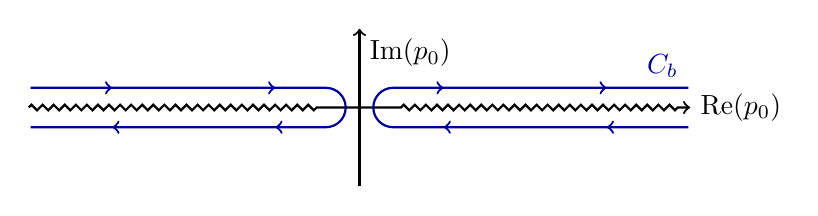
\begin{tikzpicture}[thick]

  % Axes:
  \draw [decorate,decoration={zigzag,segment length=4,amplitude=1,post=lineto,post length=15}] (-1.05*\xr,0) -- (0,0);
  \draw [->,decorate,decoration={zigzag,segment length=4,amplitude=1,pre=lineto,pre length=15,post=lineto,post length=3}] (0,0) -- (1.05*\xr,0) node [right] {$\Re(p_0)$};
  \draw [->] (0,-\yr) -- (0,\yr) node [below right] {$\Im(p_0)$};

  % Left contour line
  \draw[xshift=5,blue!60!black,decoration={markings,mark=between positions 0.125 and 0.875 step 0.25 with \arrow{>}},postaction={decorate}] (\xr,-\yr/4) -- (\yr/4,-\yr/4) arc (-90:-270:\yr/4) (\yr/4,\yr/4) -- (\xr,\yr/4) node[above left] {$C_b$};

  % Right contour line
  \draw[xshift=-5,blue!60!black,decoration={markings,mark=between positions 0.125 and 0.875 step 0.25 with \arrow{>}},postaction={decorate}] (-\xr,\yr/4) -- (-\yr/4,\yr/4) arc (90:-90:\yr/4) (-\yr/4,-\yr/4) -- (-\xr,-\yr/4);

\end{tikzpicture}
\end{document}
